% Options for packages loaded elsewhere
% Options for packages loaded elsewhere
\PassOptionsToPackage{unicode}{hyperref}
\PassOptionsToPackage{hyphens}{url}
\PassOptionsToPackage{dvipsnames,svgnames,x11names}{xcolor}
%
\documentclass[
  10pt,
  letterpaper,
  DIV=11,
  numbers=noendperiod]{scrartcl}
\usepackage{xcolor}
\usepackage{amsmath,amssymb}
\setcounter{secnumdepth}{-\maxdimen} % remove section numbering
\usepackage{iftex}
\ifPDFTeX
  \usepackage[T1]{fontenc}
  \usepackage[utf8]{inputenc}
  \usepackage{textcomp} % provide euro and other symbols
\else % if luatex or xetex
  \usepackage{unicode-math} % this also loads fontspec
  \defaultfontfeatures{Scale=MatchLowercase}
  \defaultfontfeatures[\rmfamily]{Ligatures=TeX,Scale=1}
\fi
\usepackage{lmodern}
\ifPDFTeX\else
  % xetex/luatex font selection
\fi
% Use upquote if available, for straight quotes in verbatim environments
\IfFileExists{upquote.sty}{\usepackage{upquote}}{}
\IfFileExists{microtype.sty}{% use microtype if available
  \usepackage[]{microtype}
  \UseMicrotypeSet[protrusion]{basicmath} % disable protrusion for tt fonts
}{}
\makeatletter
\@ifundefined{KOMAClassName}{% if non-KOMA class
  \IfFileExists{parskip.sty}{%
    \usepackage{parskip}
  }{% else
    \setlength{\parindent}{0pt}
    \setlength{\parskip}{6pt plus 2pt minus 1pt}}
}{% if KOMA class
  \KOMAoptions{parskip=half}}
\makeatother
% Make \paragraph and \subparagraph free-standing
\makeatletter
\ifx\paragraph\undefined\else
  \let\oldparagraph\paragraph
  \renewcommand{\paragraph}{
    \@ifstar
      \xxxParagraphStar
      \xxxParagraphNoStar
  }
  \newcommand{\xxxParagraphStar}[1]{\oldparagraph*{#1}\mbox{}}
  \newcommand{\xxxParagraphNoStar}[1]{\oldparagraph{#1}\mbox{}}
\fi
\ifx\subparagraph\undefined\else
  \let\oldsubparagraph\subparagraph
  \renewcommand{\subparagraph}{
    \@ifstar
      \xxxSubParagraphStar
      \xxxSubParagraphNoStar
  }
  \newcommand{\xxxSubParagraphStar}[1]{\oldsubparagraph*{#1}\mbox{}}
  \newcommand{\xxxSubParagraphNoStar}[1]{\oldsubparagraph{#1}\mbox{}}
\fi
\makeatother

\usepackage{color}
\usepackage{fancyvrb}
\newcommand{\VerbBar}{|}
\newcommand{\VERB}{\Verb[commandchars=\\\{\}]}
\DefineVerbatimEnvironment{Highlighting}{Verbatim}{commandchars=\\\{\}}
% Add ',fontsize=\small' for more characters per line
\usepackage{framed}
\definecolor{shadecolor}{RGB}{241,243,245}
\newenvironment{Shaded}{\begin{snugshade}}{\end{snugshade}}
\newcommand{\AlertTok}[1]{\textcolor[rgb]{0.68,0.00,0.00}{#1}}
\newcommand{\AnnotationTok}[1]{\textcolor[rgb]{0.37,0.37,0.37}{#1}}
\newcommand{\AttributeTok}[1]{\textcolor[rgb]{0.40,0.45,0.13}{#1}}
\newcommand{\BaseNTok}[1]{\textcolor[rgb]{0.68,0.00,0.00}{#1}}
\newcommand{\BuiltInTok}[1]{\textcolor[rgb]{0.00,0.23,0.31}{#1}}
\newcommand{\CharTok}[1]{\textcolor[rgb]{0.13,0.47,0.30}{#1}}
\newcommand{\CommentTok}[1]{\textcolor[rgb]{0.37,0.37,0.37}{#1}}
\newcommand{\CommentVarTok}[1]{\textcolor[rgb]{0.37,0.37,0.37}{\textit{#1}}}
\newcommand{\ConstantTok}[1]{\textcolor[rgb]{0.56,0.35,0.01}{#1}}
\newcommand{\ControlFlowTok}[1]{\textcolor[rgb]{0.00,0.23,0.31}{\textbf{#1}}}
\newcommand{\DataTypeTok}[1]{\textcolor[rgb]{0.68,0.00,0.00}{#1}}
\newcommand{\DecValTok}[1]{\textcolor[rgb]{0.68,0.00,0.00}{#1}}
\newcommand{\DocumentationTok}[1]{\textcolor[rgb]{0.37,0.37,0.37}{\textit{#1}}}
\newcommand{\ErrorTok}[1]{\textcolor[rgb]{0.68,0.00,0.00}{#1}}
\newcommand{\ExtensionTok}[1]{\textcolor[rgb]{0.00,0.23,0.31}{#1}}
\newcommand{\FloatTok}[1]{\textcolor[rgb]{0.68,0.00,0.00}{#1}}
\newcommand{\FunctionTok}[1]{\textcolor[rgb]{0.28,0.35,0.67}{#1}}
\newcommand{\ImportTok}[1]{\textcolor[rgb]{0.00,0.46,0.62}{#1}}
\newcommand{\InformationTok}[1]{\textcolor[rgb]{0.37,0.37,0.37}{#1}}
\newcommand{\KeywordTok}[1]{\textcolor[rgb]{0.00,0.23,0.31}{\textbf{#1}}}
\newcommand{\NormalTok}[1]{\textcolor[rgb]{0.00,0.23,0.31}{#1}}
\newcommand{\OperatorTok}[1]{\textcolor[rgb]{0.37,0.37,0.37}{#1}}
\newcommand{\OtherTok}[1]{\textcolor[rgb]{0.00,0.23,0.31}{#1}}
\newcommand{\PreprocessorTok}[1]{\textcolor[rgb]{0.68,0.00,0.00}{#1}}
\newcommand{\RegionMarkerTok}[1]{\textcolor[rgb]{0.00,0.23,0.31}{#1}}
\newcommand{\SpecialCharTok}[1]{\textcolor[rgb]{0.37,0.37,0.37}{#1}}
\newcommand{\SpecialStringTok}[1]{\textcolor[rgb]{0.13,0.47,0.30}{#1}}
\newcommand{\StringTok}[1]{\textcolor[rgb]{0.13,0.47,0.30}{#1}}
\newcommand{\VariableTok}[1]{\textcolor[rgb]{0.07,0.07,0.07}{#1}}
\newcommand{\VerbatimStringTok}[1]{\textcolor[rgb]{0.13,0.47,0.30}{#1}}
\newcommand{\WarningTok}[1]{\textcolor[rgb]{0.37,0.37,0.37}{\textit{#1}}}

\usepackage{longtable,booktabs,array}
\usepackage{calc} % for calculating minipage widths
% Correct order of tables after \paragraph or \subparagraph
\usepackage{etoolbox}
\makeatletter
\patchcmd\longtable{\par}{\if@noskipsec\mbox{}\fi\par}{}{}
\makeatother
% Allow footnotes in longtable head/foot
\IfFileExists{footnotehyper.sty}{\usepackage{footnotehyper}}{\usepackage{footnote}}
\makesavenoteenv{longtable}
\usepackage{graphicx}
\makeatletter
\newsavebox\pandoc@box
\newcommand*\pandocbounded[1]{% scales image to fit in text height/width
  \sbox\pandoc@box{#1}%
  \Gscale@div\@tempa{\textheight}{\dimexpr\ht\pandoc@box+\dp\pandoc@box\relax}%
  \Gscale@div\@tempb{\linewidth}{\wd\pandoc@box}%
  \ifdim\@tempb\p@<\@tempa\p@\let\@tempa\@tempb\fi% select the smaller of both
  \ifdim\@tempa\p@<\p@\scalebox{\@tempa}{\usebox\pandoc@box}%
  \else\usebox{\pandoc@box}%
  \fi%
}
% Set default figure placement to htbp
\def\fps@figure{htbp}
\makeatother





\setlength{\emergencystretch}{3em} % prevent overfull lines

\providecommand{\tightlist}{%
  \setlength{\itemsep}{0pt}\setlength{\parskip}{0pt}}



 


\usepackage{etoolbox}
\usepackage{hyperref}
\KOMAoption{captions}{tableheading}
\makeatletter
\@ifpackageloaded{caption}{}{\usepackage{caption}}
\AtBeginDocument{%
\ifdefined\contentsname
  \renewcommand*\contentsname{Table of contents}
\else
  \newcommand\contentsname{Table of contents}
\fi
\ifdefined\listfigurename
  \renewcommand*\listfigurename{List of Figures}
\else
  \newcommand\listfigurename{List of Figures}
\fi
\ifdefined\listtablename
  \renewcommand*\listtablename{List of Tables}
\else
  \newcommand\listtablename{List of Tables}
\fi
\ifdefined\figurename
  \renewcommand*\figurename{Figure}
\else
  \newcommand\figurename{Figure}
\fi
\ifdefined\tablename
  \renewcommand*\tablename{Table}
\else
  \newcommand\tablename{Table}
\fi
}
\@ifpackageloaded{float}{}{\usepackage{float}}
\floatstyle{ruled}
\@ifundefined{c@chapter}{\newfloat{codelisting}{h}{lop}}{\newfloat{codelisting}{h}{lop}[chapter]}
\floatname{codelisting}{Listing}
\newcommand*\listoflistings{\listof{codelisting}{List of Listings}}
\makeatother
\makeatletter
\makeatother
\makeatletter
\@ifpackageloaded{caption}{}{\usepackage{caption}}
\@ifpackageloaded{subcaption}{}{\usepackage{subcaption}}
\makeatother
\usepackage{bookmark}
\IfFileExists{xurl.sty}{\usepackage{xurl}}{} % add URL line breaks if available
\urlstyle{same}
\hypersetup{
  pdftitle={CDC BRFSS Analysis: Veteran Health},
  pdfauthor={Math 62 - Spring 2026},
  colorlinks=true,
  linkcolor={blue},
  filecolor={Maroon},
  citecolor={Blue},
  urlcolor={Blue},
  pdfcreator={LaTeX via pandoc}}


\title{CDC BRFSS Analysis: Veteran Health}
\author{Elsa Li, Amanda Louie, Anika Sharma}
\date{}
\begin{document}
\maketitle


\section{Introduction}\label{introduction}

Veterans make up about 15.8 million people, as of 2023, as part of the
US population (US Census Bureau 2022). Health policies surrounding
veterans are often a political issue that needs addressing as veterans
serving experience impacts their health and a lack of support and access
to their health benefits when they come back from their service affects
their physical and mental wellbeing. According to National Veterans
Homeless Support, ``During the period from 2001 to 2020, the frequency
of mental health issues and substance use disorders among Veterans
Health Administration (VHA) participants increased significantly, from
27.9\% to 41.9\%. Veterans face a heightened risk of suicide, being 1.5
times more likely than civilians'' (NVHS). We were particularly
interested in investigating and characterizing the health of veterans in
depth. Hence, this report is centered around the broader issue of
veteran well-being. We will use the BRFSS 2022 dataset, which is a
survey of risk assessment factors conducted by the CDC in the general US
population (CDC 2022), to investigate veteran well-being in detail. The
key categories that we will be exploring are:

\begin{enumerate}
\def\labelenumi{\arabic{enumi}.}
\tightlist
\item
  How do the demographics of the veteran population differ from the
  national distribution?
\item
  How is veteran status associated with individuals' physical health and
  mental health?
\item
  What are some factors that influence both mental and physical health
  amongst veterans?
\end{enumerate}

In answering these questions and henceforth further unpacking the
current state of veteran well-being, we hope we can make concrete and
statistically backed claims to guide policy which better supports
veterans in access, equity, and welfare. Note that all the claims and
analysis we make are based on this BRFSS dataset only, and should not be
extrapolated beyond without further statistical analysis.

\section{Demographics}\label{demographics}

When thinking about veterans in the larger context of this dataset, we
were first interested in exploring \emph{who} the veterans in the United
States are. This question is important because in order to support
veteran well-being we need to first understand what their demographic
background is. The first step we took was to conduct exploratory data
analysis on the veteran sample within the BRFSS dataset. Some notable
findings we found were that 88.6\% of veterans are men, the majority
race is White-only, non Hispanic --- making up 81.3\% of the sample,
43.1\% of veterans are college graduates, and 17.2\% of veterans are 80
or older.

These results motivated the key guiding question: how do the
demographics of veterans differ from the general population? To
investigate this, we conducted a Chi-squared goodness of fit test which
compared the distributions of the demographics of veterans to that of
the national distribution. By demographics, here we chose to include:
race, education level, and income level --- we conducted separate tests
for each one of these. The national average data was taken from census
bureau data collected in 2022 (USAFacts 2026). The null hypothesis for
the Chi-squared goodness of fit test is that the veteran sample follows
the same distribution as the national average and the alternative
hypothesis is that the veteran sample does not follow the same
distribution as the national average.

Let's consider the assumptions of a Chi-squared test. First, we assume
that there is independence between outcomes. This means that data points
aren't paired, and are independent of one another. Since the BRFSS
dataset comes from a large sampled survey, we can assume random sampling
where each respondent's answers is independent of others. The second
assumption is that the sample size must have at least 5 expected cases.
This is true for all the demographic variables since we have
\(n = 42841\), so the expected counts \((n \times\) expected
proportion). is always larger than 5. The last condition is that
\(df  = k-1 > 1\) (where \(k\) is the number of categories) which holds
since we have more than 2 categories for each of our demographic
variables. Hence, all the conditions are met.

After conducting a Chi-squared test, we found that in each case (race,
education, and income) the results were significant at a 95\% confidence
level --- meaning that the p-value was below 0.05. Hence, we
investigated further to see which groups differed the most using
multiple 1-sample proportion tests with adjusted p-values using the
Bonferroni correction. This test (along with the same independence
assumption stated above) assumes that \(Z \sim N(0,1)\) meaning that the
Z-distribution can be approximated by the normal distribution. This is
true when \(np_0 \geq 10\) and \(n(1-p_0) \geq 10\). Since
\(n = 42841\), this condition holds for all our values of \(p_0\) in
each of race, education level, and income level. The results for each of
the tests is shown below:

\begin{table}[h]
\centering
\renewcommand{\arraystretch}{0.8}
\begin{tabular}{lrrrl}
\toprule
Race & \makecell{Veteran\\Prop.} & \makecell{National\\Prop.} & \makecell{p-value\\(adj)} & Direction \\
\midrule
Asian only, non-Hispanic & 0.0127 & 0.0610 & $< 2.2\mathrm{e}{-16}$ & Underrepresented \\
Hispanic & 0.0500 & 0.1910 & $< 2.2\mathrm{e}{-16}$ & Underrepresented \\
White only, non-Hispanic & 0.8132 & 0.5890 & $< 2.2\mathrm{e}{-16}$ & Overrepresented \\
Black only, non-Hispanic & 0.0743 & 0.1260 & $< 2.2\mathrm{e}{-16}$ & Underrepresented \\
American Indian or Alaskan Native only, Non-Hispanic & 0.0171 & 0.0070 & $< 2.2\mathrm{e}{-16}$ & Overrepresented \\
Native Hawaiian or other Pacific Islander only, Non-Hispanic & 0.0063 & 0.0020 & $< 2.2\mathrm{e}{-16}$ & Overrepresented \\
Multiracial, non-Hispanic & 0.0264 & 0.0240 & $1.16 \times 10^{-2}$ & Overrepresented \\
\bottomrule
\end{tabular}
\end{table}

\begin{center}

\textbf{Figure 1:} 1-sample proportion test between the national average and the sampled veteran population (race)

\end{center}

\begin{table}[h]
\centering
\renewcommand{\arraystretch}{0.8}
\begin{tabular}{lrrrl}
\toprule
Education & Observed\_Prop & Expected\_Prop & p\_bonferroni & Direction \\
\midrule
Less than high school & 0.02516292 & 0.1088911 & 0.000000e+00 & Underrepresented \\
Bachelor's or higher & 0.42279884 & 0.3426573 & 4.203017e-262 & Overrepresented \\
Some college / associate & 0.32483470 & 0.2847153 & 1.206677e-73 & Overrepresented \\
High school graduate & 0.22720354 & 0.2637363 & 3.298299e-64 & Underrepresented \\
\bottomrule
\end{tabular}
\end{table}

\begin{center}

\textbf{Figure 2:} 1-sample proportion test between the national average and the sampled veteran population (education)

\end{center}

\begin{table}[h]
\centering
\renewcommand{\arraystretch}{0.8}
\begin{tabular}{lrrrl}
\toprule
Income & Observed\_Prop & Expected\_Prop & p\_bonferroni & Direction \\
\midrule
\$25,000 to less than \$50,000 & 0.2661385 & 0.171 & 0.000000e+00 & Overrepresented \\
\$75,000 or more & 0.4214797 & 0.520 & 7.461731e-310 & Underrepresented \\
\$50,000 to less than \$75,000 & 0.2022149 & 0.148 & 2.430662e-186 & Overrepresented \\
Less than \$25,000 & 0.1101669 & 0.161 & 3.483507e-153 & Underrepresented \\
\bottomrule
\end{tabular}
\end{table}

\begin{center}

\textbf{Figure 3:} 1-sample proportion test between the national average and the sampled veteran population (income level).

\end{center}

In all of these cases, we can see that the adjusted p-values are still
well under 0.05. Hence this suggests that there is statistically
significant evidence that the population proportion is different from
the expected value for each group. We also compute the direction of the
difference: some groups are underrepresented whereas others are
overrepresented. Through this we see some expected trends following our
exploratory analysis. For example, the group White only-non hispanic is
overrepresented. Although we also see some perhaps counterintuitive
trends. For example, the group of Bachelor's or higher education level
is overrepresented, but the group earning \$75k or more is
underrepresented. It's important to note also that statistical
significance doesn't always translate to practical significance. An
example of this is in the race demographic where the value we observed
for Multiracial, non-Hispanic was 0.026, and what we expected was 0.024
--- which practically may not be significant. Also, since the sampled
veteran population is skewed in terms of some demographic factors (Eg:
veterans in this dataset are much older than the general population),
the comparison to the entire US population data should be treated with
caution.

Overall, we can conclude that the demographics of the veteran population
differ from the national population, and it motivates the next question:
how might these demographic differences affect comparisons of health
outcomes between veterans and non-veterans?

\section{Physical and Mental Health in Veterans
vs.~Non-Veterans}\label{physical-and-mental-health-in-veterans-vs.-non-veterans}

We looked how being a veteran affects the likelihood of being
susceptible to certain physical and mental health factors. The
significance of this test determines whether we believe health policies
should vary between veterans and non-veterans. In order to do this, we
ran proportion comparison z-tests and a two-sample mean comparison
t-test between the veterans and non-veterans that experience certain
physical and mental health factors. The results of our comparison tests
are discussed in the following sections.

\subsection{Physical Health
Comparisons}\label{physical-health-comparisons}

In our comparison tests, which were two-sample proportion z-tests and a
two-sample mean comparison test, our proposed null hypothesis is that
the proportion of veterans that experience specific physical health
factors was not different from the proportion of non-veterans who
experience the same factors (\(H_0: p_{veteran} = p_{nonveteran}\),
\(H_A: p_{veteran} \neq p_{nonveteran}\)).For the category
\texttt{daysphyshlthnotgood}, participants reported the number of days
in the past month where their physical health was not good and so we
compared the means in this case instead.

The assumptions we made while conducting our comparison tests were that
the veterans and non-veterans datasets are independent and individual
people are independent from each other. These conditions are both
satisfied since being a veteran is independent of being a non-veteran
and each participant in the dataset answered the survey independent of
each other. Another assumption that our proportion comparison tests made
was that the success--failure condition, \(np ≥ 10\) and
\(n(1-p) ≥ 10\), was satisfied, where n is the size of the sample and p
is the proportion. For this dataset and proportions the success-failure
condition was satisfied since for all of the proportions used in this
test multiplying the proportion and 1 minus the proportion by the sample
size, as determined in section 1, would result in a number larger than
10. Two additional assumptions our mean comparison test made were that
the sample means were normally distributed among veterans and
non-veterans and that the datasets had equal variances. The first
assumption is satisfied by the Central Limit Theorem and the sizes of
each dataset as defined in section 1, leading us to conclude that the
sample means are normally distributed. We checked the second assumption
by plotting a histogram of the ``daysphyshlthnotgood'' for veteran and
non-veterans and got the following plots with similar spread of data,
which led us to believe that the variances were equal. In our initial
testing, we conducted our comparison tests with equal and unequal
variances and found that we came to the same conclusion about the
significance of any difference in the means through both tests.

\begin{center}
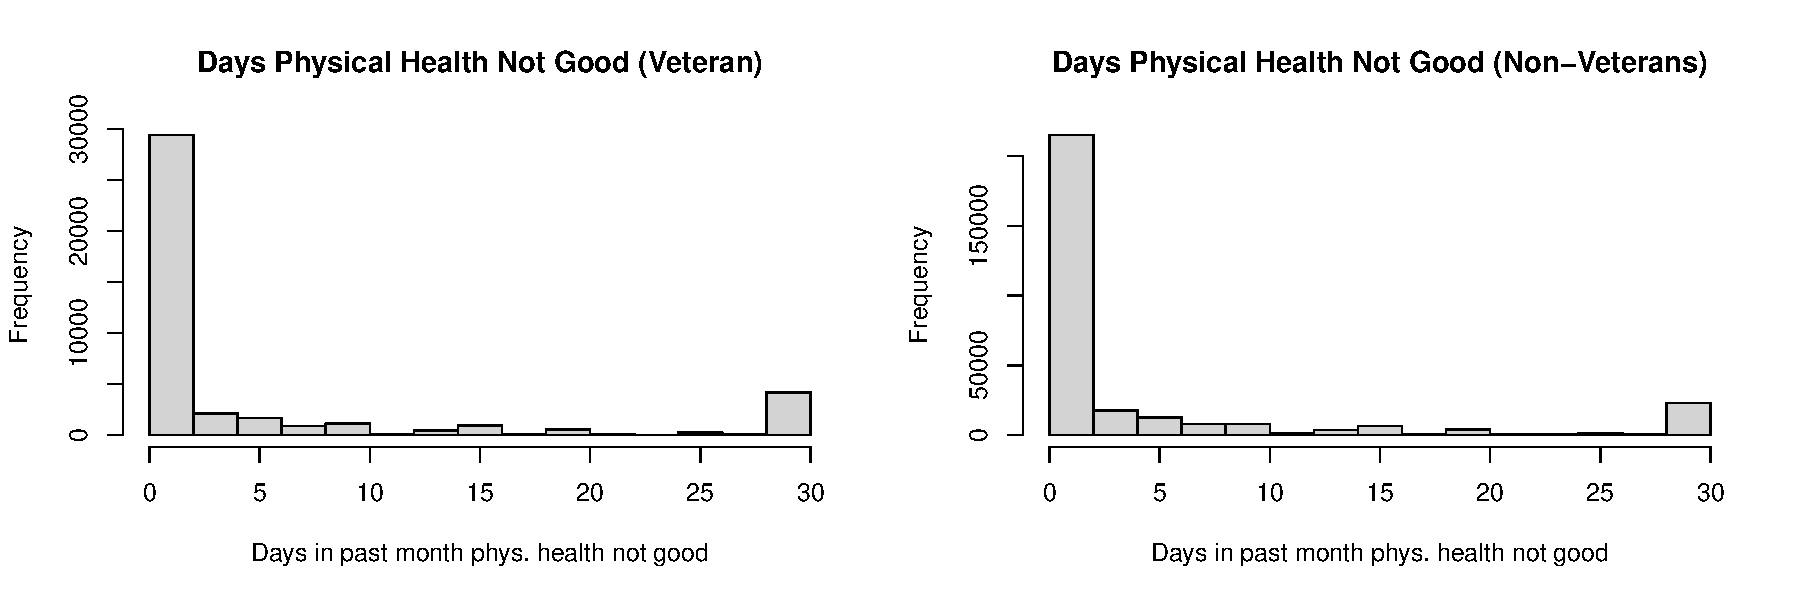
\includegraphics[width=0.6\linewidth,height=\textheight,keepaspectratio]{final-project_files/figure-pdf/unnamed-chunk-2-1.pdf}
\end{center}

\begin{center}
\textbf{Figure 4:} Histograms of the distribution of `daysphyshlthnotgood` in veterans and non-veterans to visualize variance among datasets
\end{center}

The results of our t-tests are summarized in the table below.

\begin{table}[h]
\centering
\renewcommand{\arraystretch}{0.8}
\begin{tabular}{lccc}
\toprule
Factor & Veteran & Non-Veteran & $p$-value \\
\midrule
Arthritis & 0.4356422 & 0.3455287 & $< 2.2 \times 10^{-16}$ \\
Heart Disease & 0.1244373 & 0.0543102 & $< 2.2 \times 10^{-16}$ \\
Cancer & 0.1789827 & 0.1105903 & $< 2.2 \times 10^{-16}$ \\
Diabetes & 0.1962027 & 0.1340290 & $< 2.2 \times 10^{-16}$ \\
COPD & 0.11969946 & 0.07724301 & $< 2.2 \times 10^{-16}$ \\
Days Physical Health Not Good & 4.972634 & 4.338173 & $< 2.2 \times 10^{-16}$ \\
\bottomrule
\end{tabular}
\end{table}

\begin{center}
\textbf{Figure 5:} Results of comparison tests between veterans and non-veterans on different physical health factors
\end{center}

From these comparison tests, we can conclude that there is a significant
difference in the proportions (and mean) of these physical health
factors present in veterans versus non-veterans. All of our comparison
tests resulted in a p-value less than \(2.2 \times 10^-16\), which
indicates that we would reject our null hypothesis that the proportions
or means are equal. We notice that in general the proportion of veterans
who are diagnosed with these physical health factors is greater than the
proportion of non-veterans diagnosed with the same physical health
factors. We can visualize this difference in this barplot that compares
the different proportions among veterans and non-veterans.

\begin{center}
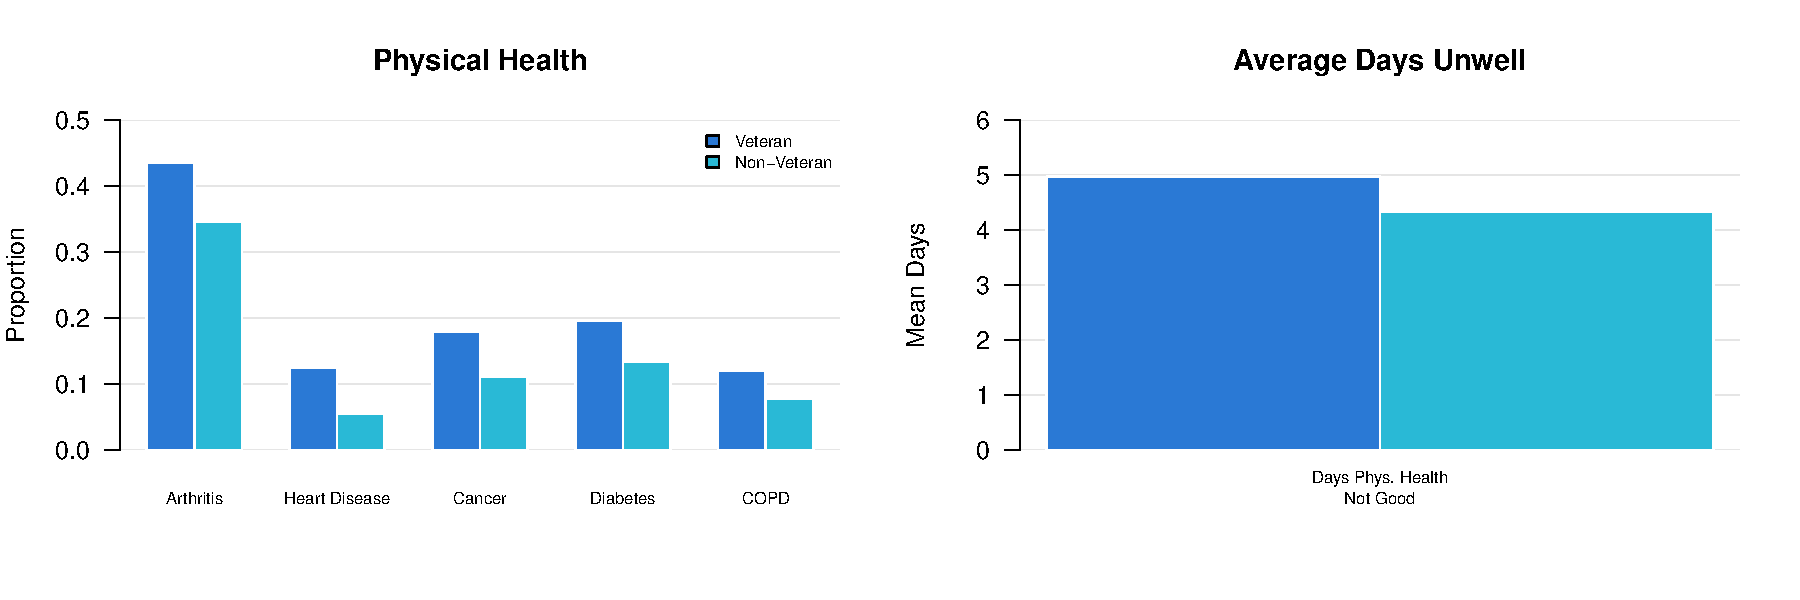
\includegraphics[width=0.6\linewidth,height=\textheight,keepaspectratio]{final-project_files/figure-pdf/unnamed-chunk-3-1.pdf}
\end{center}

\textbf{Figure 6:} Differences in proportions between veterans and non-veterans on different physical health factors

\subsection{Mental Health Comparisons}\label{mental-health-comparisons}

We proposed was the same comparison tests for mental health as for
physical health factors
\((H_0: p_{veteran} = p_{nonveteran}, H_A: p_{veteran} \neq p_{nonveteran})\).
The assumptions made in the proportion and mean comparison test were the
same and verified the same way. To verify that the datasets had equal
variances we plotted a histogram of the \texttt{daysmenthlthnotgood} for
veteran and non-veterans and got plots with similar spread of data,
which led us to believe that the variances were equal. In our initial
testing, we conducted our two-sample t-tests with equal and unequal
variances and found that we came to the same conclusion about the
significance of any difference in the means through both tests.

\begin{center}
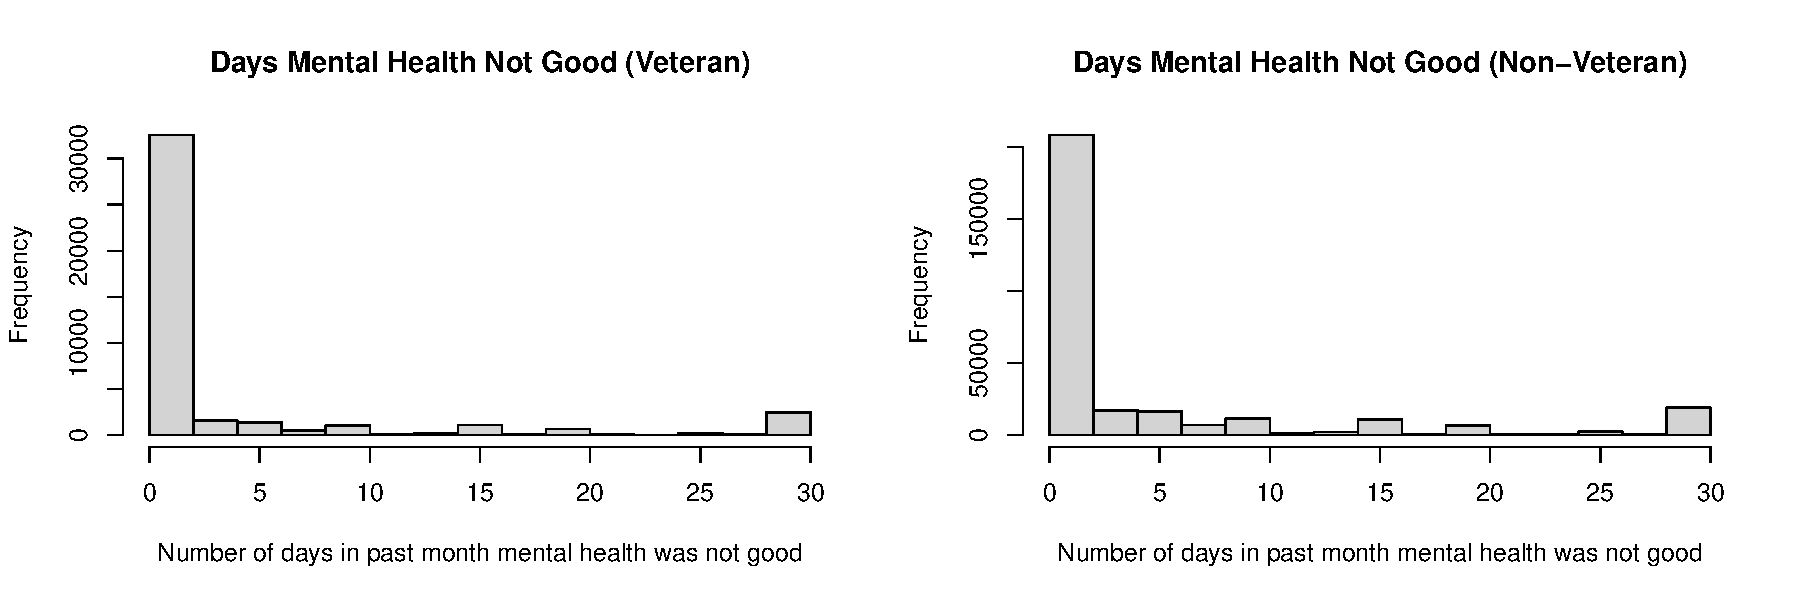
\includegraphics[width=0.6\linewidth,height=\textheight,keepaspectratio]{final-project_files/figure-pdf/unnamed-chunk-4-1.pdf}
\end{center}

\begin{center}
\textbf{Figure 7:} Histograms of the distribution of “daysmenthlthnotgood” in veterans and non-veterans to visualize variance among datasets
\end{center}

The results of our comparison tests are summarized in the table below.

\begin{table}[h]
\centering
\renewcommand{\arraystretch}{0.8}
\begin{tabular}{lccc}
\toprule
Factor & Veteran & Non-Veteran & $p$-value \\
\midrule
Depression & 0.1757344 & 0.2166535 & $< 2.2 \times 10^{-16}$ \\
Days Mental Health Not Good & 3.517690 & 4.462462 & $< 2.2 \times 10^{-16}$ \\
\bottomrule
\end{tabular}
\end{table}

\begin{center}
\textbf{Figure 8:} Differences in proportions between veterans and non-veterans on different mental health factors
\end{center}

Similarly to physical health, from these tests we can conclude that
there is a significant difference in the proportion of veterans and the
proportion of non-veterans who have been diagnosed with a depressive
disorder. Each of our comparison tests resulted in a p-value less than
\(2.2 \times 10^-16\), which indicates that we would reject our null
hypothesis that the proportions or means are the same. We can notice
that in general, unlike with the physical health factors, the proportion
of veterans who are diagnosed with a depressive disorder is less than
the proportion of non-veterans diagnosed with a depressive disorder. We
can visualize this difference in this barplot that compares the
different proportions among veterans and non-veterans.

\begin{center}
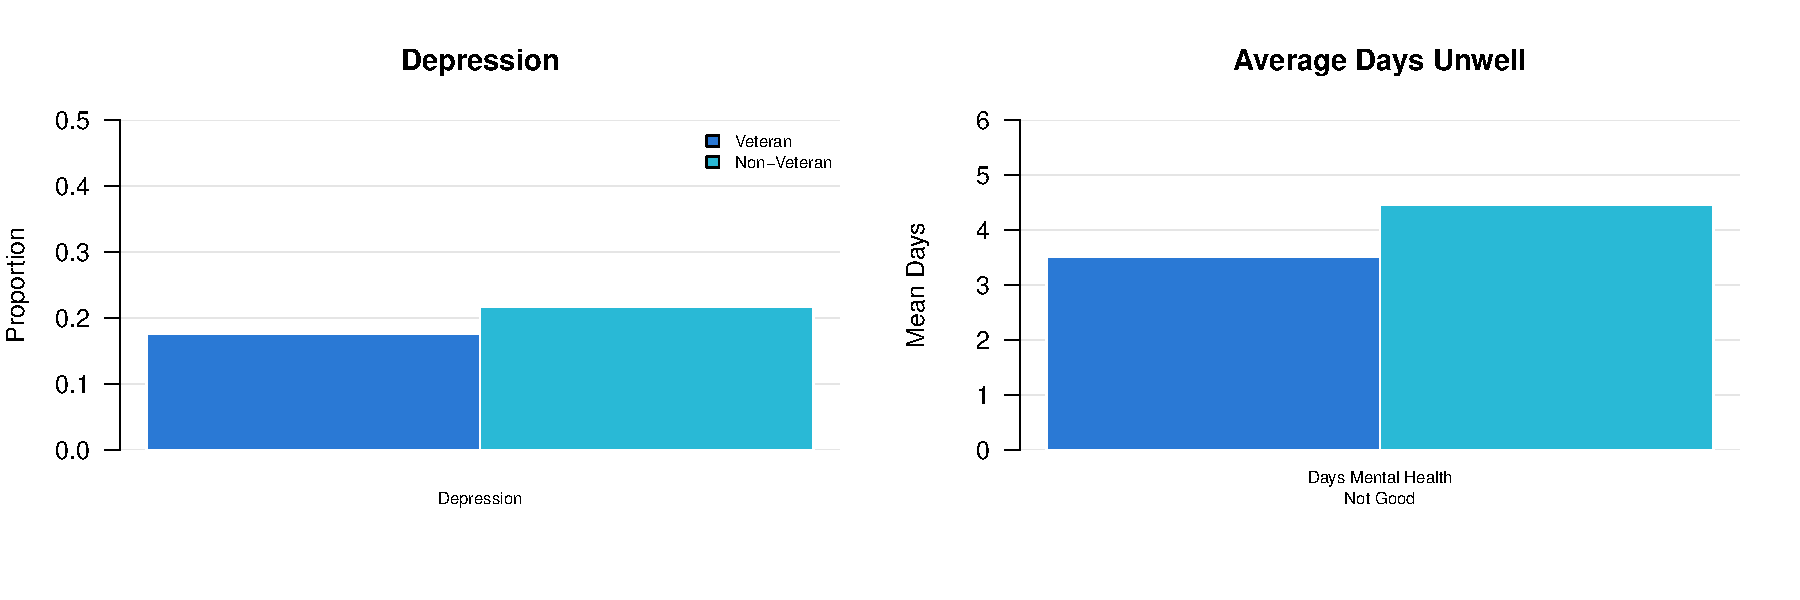
\includegraphics[width=0.6\linewidth,height=\textheight,keepaspectratio]{final-project_files/figure-pdf/unnamed-chunk-5-1.pdf}
\end{center}

\begin{center}
\textbf{Figure 9:} Differences in proportions between veterans and non-veterans on different mental health factors
\end{center}

\section{Factors Affecting Physical and Mental Health of
Veterans}\label{factors-affecting-physical-and-mental-health-of-veterans}

Within the veteran population, we were interested in finding out what
makes veterans prone to poor mental and physical health, which would
inform measures to support veteran wellbeing effectively. For the
physical health of veterans, we were most interested in finding the
factors that significantly predict the likelihood of cancer, heart
disease, diabetes, and BMI. Cancer, heart disease, and diabetes are all
binary variables, so we modeled them using logistic regression. Since
BMI is a numerical variable, we modelled it using a multiple linear
regression model. The null hypothesis for both the logistic regressions
and the linear regression are the same: for each predictor \(x_i\), the
corresponding \(\beta_i = 0\), where \(\beta_i\) is the coefficient to
\(x_i\), in the regression model. The alternative hypothesis for the
regression models is also the same: There is at least one predictor
\(x_i\), for which the corresponding \(\beta_i \neq 0\), where
\(\beta_i\) is the coefficient to \(x_i\), in the regression model.

To narrow down predictors for each model, we choose a set of predictors
that we believed would most significantly attribute to whatever the
model was trying to predict. Although we could have used the stepwise
function to eliminate those predictors that were not significant for
predicting depressive disorder, we decided against doing so. This is
because p-values and confidence intervals may no longer be valid after
running the stepwise selection function, and we wanted to interpret the
model using these features of the output. Additionally, we modified the
age column to consolidate age into either young adult, middle age, and
senior, and the income columns into either low, middle, or high income.
For heart disease, cancer, and diabetes, our chosen set of predictors
was \texttt{sex}, \texttt{bmi}, \texttt{income},
\texttt{daysphyshlthnotgood}, \texttt{anyexer}, \texttt{race},
\texttt{age}, \texttt{bingedrinker}, and \texttt{weeklydrinks}. For BMI,
our set was the same just without the BMI predictor.

We can begin with the results for our physical health models, starting
with heart disease. Note that we are only displaying the predictors that
had a significant adjusted p-value based on the Bonferroni correction.
Since we're using so many predictors, we decided to use this higher
confidence level. One interesting result we observe here is that,
keeping all other predictors constant, the odds of a male veteran having
heart disease is about 2.23 times higher to that of a female veteran.

\begin{table}[h]
\centering
\renewcommand{\arraystretch}{0.8}
\begin{tabular}{l r r r}
\toprule
\textbf{Heart Disease Predictor} & Coefficient & p\_value & Odds\_Ratio \\
\midrule
(Intercept) & -4.38013938 & 1.030130e-94 & 0.01252361 \\
sexMale & 0.80261851 & 3.610160e-20 & 2.23137617 \\
bmi & 0.02059709 & 3.387576e-10 & 1.02081067 \\
incomelow income & 0.25661775 & 5.575626e-04 & 1.29255095 \\
daysphyshlthnotgood & 0.03581590 & 9.450336e-106 & 1.03646502 \\
anyexerYes & -0.18493519 & 5.283247e-06 & 0.83115815 \\
raceNative Hawaiian or other Pacific Islander only, Non-Hispanic & 0.68088540 & 7.775356e-03 & 1.97562618 \\
agesenior & 1.23859720 & 1.724281e-138 & 3.45076934 \\
ageyoung adult & -2.24758619 & 1.018028e-19 & 0.10565395 \\
bingedrinkerYes & -0.22273369 & 7.370868e-03 & 0.80032796 \\
weeklydrinks & -0.01068126 & 8.289779e-04 & 0.98937558 \\
\bottomrule
\end{tabular}
\end{table}

For cancer, we note that some interesting results are that being a
senior was again an especially important for predicting cancer, as it
raised the odds of a senior having cancer was about 3.54 times more
likely than the reference group of middle aged, when keeping all other
predictors constant.

\begin{table}[h]
\centering
\renewcommand{\arraystretch}{0.8}
\begin{tabular}{l r r r}
\toprule
\textbf{Cancer Predictor} & Coefficient & p\_value & Odds\_Ratio \\
\midrule
(Intercept) & -2.03178780 & 2.882294e-30 & 0.1311009 \\
bmi & -0.01243622 & 3.430060e-05 & 0.9876408 \\
daysphyshlthnotgood & 0.02221518 & 1.349809e-46 & 1.0224638 \\
raceAsian only, non-Hispanic & -0.94885042 & 1.690569e-04 & 0.3871859 \\
agesenior & 1.31578327 & 4.803320e-215 & 3.7276696 \\
ageyoung adult & -1.28756612 & 5.411407e-24 & 0.2759416 \\
bingedrinkerYes & -0.27515240 & 1.761594e-05 & 0.7594564 \\
incomelow income & -0.23173324 & 1.067433e-04 & 0.7931577 \\
\bottomrule
\end{tabular}
\end{table}

Once again, being a senior was a significant contributor to having
diabetes. Additionally, being a Native Hawaiian or other Pacific
Islander increased a participating veteran's odds of having diabetes by
about 2.06 times versus the reference race of American Indian or Alaska
Native, when keeping all other predictors constant.

\begin{table}[h]
\centering
\renewcommand{\arraystretch}{0.8}
\begin{tabular}{l r r r}
\toprule
\textbf{Diabetes Predictor} & Coefficient & p\_value & Odds\_Ratio \\
\midrule
(Intercept) & -4.52351385 & 7.071627e-171 & 0.01085083 \\
sexMale & 0.50020112 & 1.150702e-17 & 1.64905289 \\
bmi & 0.08699755 & 5.699442e-218 & 1.09089400 \\
incomelow income & 0.49233993 & 2.041857e-15 & 1.63614020 \\
incomemedium income & 0.33029307 & 4.967705e-09 & 1.39137584 \\
daysphyshlthnotgood & 0.02216352 & 1.309265e-50 & 1.02241096 \\
anyexerYes & -0.37677571 & 8.668877e-29 & 0.68606993 \\
raceWhite only, non-Hispanic & -0.44906561 & 4.238654e-05 & 0.63822422 \\
agesenior & 0.75707326 & 1.324741e-98 & 2.13202719 \\
ageyoung adult & -2.33914218 & 5.979166e-58 & 0.09641031 \\
bingedrinkerYes & -0.20653020 & 2.002169e-03 & 0.81340170 \\
weeklydrinks & -0.02587227 & 7.107947e-17 & 0.97445955 \\
\bottomrule
\end{tabular}
\end{table}

Again, being a senior or being a Native Hawaiian or other Pacific
Islander increased a participating veteran's predicted BMI compared to
the reference race of American Indian or Alaska Native, when holding all
other predictors constant.

\begin{table}[h]
\centering
\renewcommand{\arraystretch}{0.8}
\begin{tabular}{l r r r}
\toprule
\textbf{BMI Predictor} & Coefficient & p\_value \\
\midrule
(Intercept) & 30.11042063 & 0.000000e+00 \\
sexMale & 0.58101745 & 5.184119e-09 \\
incomemedium income & 0.45076399 & 2.949942e-06 \\
daysphyshlthnotgood & 0.03496438 & 3.582552e-25 \\
anyexerYes & -1.35134430 & 1.732838e-74 \\
raceAsian only, non-Hispanic & -2.29296896 & 1.295361e-10 \\
agesenior & -1.91867928 & 1.211723e-165 \\
ageyoung adult & -1.11652855 & 2.464129e-24 \\
bingedrinkerYes & 0.37072697 & 3.320259e-04 \\
weeklydrinks & -0.02155940 & 6.859478e-12 \\
\bottomrule
\end{tabular}
\end{table}

We can conclude by checking the assumptions for the logistic regression
model. First, we assume that the observations in our dataset are
independent. Since this BRFSS dataset is made up of randomly chosen
respondents from all over the United States, we can assume that the
veterans in the dataset are all independent of each other as well. The
total number of veterans in the BRFSS dataset is 42841, and the number
of veterans is also greater than 32000 within each of the factors we
examined, so our sample size is sufficiently large. Lastly, we also
assume that the logistic odds of success are linear in the predictors.
Since we were not given the statistical tools to validate this
assumption, we will not verify this assumption in this report, but note
that our conclusions may have type I error where we rejected the null
hypothesis despite it being true.

Next, we can check the assumptions for the multiple linear regression
model. Our assumptions are that the linear model holds, the errors are
independent of each other, and the sample mean error is normally
distributed. From the residual plots in Fig 10, we can see that our
assumption does not hold, since there seems to be a lot more residuals
above the red line, and most residuals are clustered towards higher
fitted values. From the Q-Q plot, we can see a distinct right tail,
which also suggests that residuals are not normally distributed.
However, we also know that the central limit theorem applies because our
sample size is large, but we must still interpret any final output of
the linear model with caution.

\begin{center}
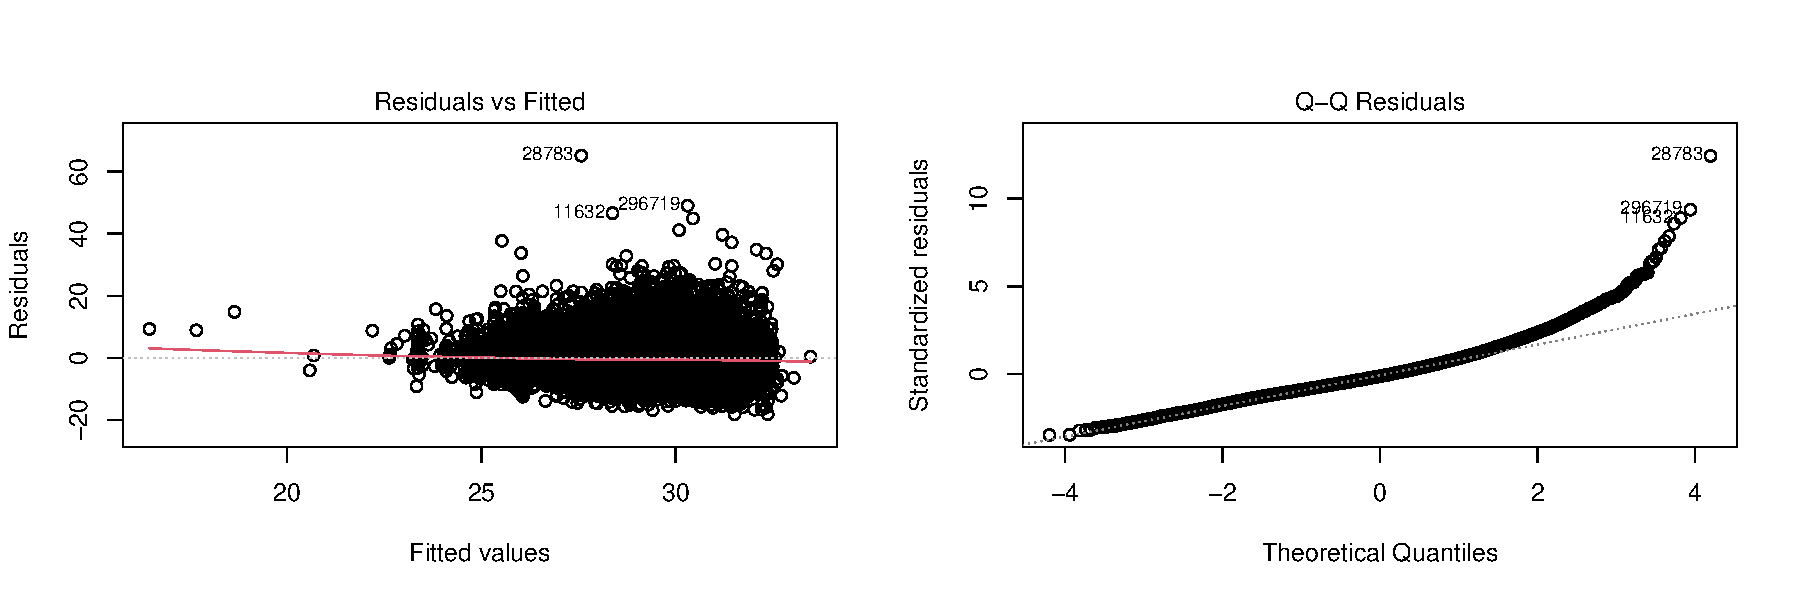
\includegraphics[width=0.6\linewidth,height=\textheight,keepaspectratio]{final-project_files/figure-pdf/unnamed-chunk-6-1.pdf}
\end{center}

\begin{center}
\textbf{Figure 10} Residuals Plots of BMI linear regression model 
\end{center}

\section{Factors Affecting Mental
Health}\label{factors-affecting-mental-health}

For the mental health of veterans, we decided to focus on whether or not
they have been told that they have a depressive disorder. Similar to how
we conducted the data analysis, we ran a logistic regression model with
some preselected predictors. This time, we chose our predictors to be
\texttt{sex}, \texttt{income}, \texttt{race}, \texttt{age},
\texttt{bingedrinker}, \texttt{weeklydrinks},
\texttt{daysmenthlthnotgood}, and \texttt{anyexer}. From the results of
the model, we can see that lower income veterans were around 1.9 times
more likely to have been told that they have a depressive disorder than
the reference group of high income veterans, holding all other
predictors constant.

\begin{table}[h]
\centering
\renewcommand{\arraystretch}{0.8}
\begin{tabular}{l r r r}
\toprule
\textbf{Depression Predictor} & Coefficient & p\_value & Odds\_Ratio \\
\midrule
(Intercept) & -1.2856906 & 9.250189e-21 & 0.2764596 \\
sexMale & -0.8586733 & 6.026534e-85 & 0.4237238 \\
incomelow income & 0.6356814 & 2.922495e-23 & 1.8883083 \\
incomemedium income & 0.3306027 & 7.745822e-09 & 1.3918067 \\
daysmenthlthnotgood & 0.1072040 & 0.000000e+00 & 1.1131613 \\
anyexerYes & -0.2058627 & 5.118803e-08 & 0.8139448 \\
agesenior & -0.5226292 & 1.694792e-44 & 0.5929595 \\
\bottomrule
\end{tabular}
\end{table}

Lastly, we can verify our assumptions about this model. Since this is
just a logistic regression model, the same assumptions about sample size
and logistic odds of success being linear in the predictors hold.

\section{Conclusions and
Recommendations}\label{conclusions-and-recommendations}

From the results of all of the above models we gain a number of key
insights. Although before we get into the results, we'd like to restate
that all these conclusions should be interpreted only within the context
of the BRFSS dataset and cannot be extrapolated beyond without further
analysis.

From the initial demographic section we learned that the demographics of
veterans are statistically different from the general US population in
income, education and race. Certain races (Black, Hispanic, and Asians)
were underrepresented in the veteran population, whilst others are
overrepresented --- such as White-only non-Hispanic. This could inform
health policy and staff to be more prepared for diseases which put
certain races at higher-risk than others.

In the second section, we unpacked how given a particular health factor,
the difference in proportion of veterans and non-veteran who have it is
statistically significant. In particular, for physical health factors
(heart disease, diabetes, cancer, BMI), we found that veterans are more
likely to have the factor. Whereas, for depression, non-veterans are
more likely to have it. Hence, this could inform health policy to guide
more targeted attention for the physical health of veterans through
prevention and holistic well-being support. In contrast, the mental
health policies should remain broad and be catered to both the general
population and veterans.

In the last section, we further examined the factors that impact
veterans' physical and mental health. An unsurprising result is that
being a senior almost always increases a veteran's odds of health issues
the most. Additionally, we repeatedly found that being a Native Hawaiian
or other Pacific Islander increased odds of having multiple health
conditions. We also found that for mental health issues, lower income
veterans were more likely to have been told that they have a depressive
disorder. Therefore, we suggest allocating more physical health
resources to the older veteran and Native Hawaiian and other Pacific
Islander population, and allocate more mental health resources to lower
income veteran communities.

\newpage

\subsection{Bibliography}\label{bibliography}

Bureau, US Census. ``Veterans Day 2024: November 11.'' Census.gov, 16
Oct.~2024,
www.census.gov/newsroom/facts-for-features/2024/veterans-day.html.CDC.

``CDC - BRFSS Annual Survey Data.'' Www.cdc.gov, 31 Aug.~2020,
www.cdc.gov/brfss/annual\_data/annual\_data.htm.USAFacts.

``How Many People Live in the US?'' USAFacts, 4 Mar.~2026,
usafacts.org/answers/how-many-people-live-in-the-us/country/united-states/.

``Understanding Veterans and Mental Illness.'' NVHS, 16 Apr.~2026,
nvhs.org/veterans-and-mental-illness/?gad\_source=1\&gad\_campaignid=15514416182\&gbraid=0AAAAADmTLu
\_p7ZVXVkF4UyN7N9n5jjY9F\&gclid=Cj0KCQjwkrzPBhCqARIsAJN460n3DcDuNSRaDDfYjG504YRMtHBaX3T7JY9CyThlfLlgCba47os4apEaAhUjEALw\_wcB.

\subsection{Appendix}\label{appendix}

Below is all the code we used to complete tests and generate models. All
graphs and tables come from the code from here.

\section{Team Members}\label{team-members}

Li, Elsa

Louie, Amanda

Sharma, Anika

\begin{center}\rule{0.5\linewidth}{0.5pt}\end{center}

\begin{Shaded}
\begin{Highlighting}[]
\DecValTok{2} \SpecialCharTok{*} \DecValTok{2}
\end{Highlighting}
\end{Shaded}

\begin{verbatim}
[1] 4
\end{verbatim}

The \texttt{echo:\ true} option enables the printing of code (only
output is displayed).

Amanda Section

\begin{verbatim}
[1] 42841
\end{verbatim}

\begin{verbatim}
[1] 309572
\end{verbatim}

Comparisons of physical health between veterans and non-veterans:

Arthritis: p-value \(< 2.2 \times 10^{-16}\)

\begin{verbatim}

    2-sample test for equality of proportions with continuity correction

data:  successes out of n_obs
X-squared = 1324, df = 1, p-value < 2.2e-16
alternative hypothesis: two.sided
95 percent confidence interval:
 0.08510047 0.09512656
sample estimates:
   prop 1    prop 2 
0.4356422 0.3455287 
\end{verbatim}

Heart Disease: p-value \(< 2.2 \times 10^{-16}\)

\begin{verbatim}

    2-sample test for equality of proportions with continuity correction

data:  successes out of n_obs
X-squared = 3099.4, df = 1, p-value < 2.2e-16
alternative hypothesis: two.sided
95 percent confidence interval:
 0.06686406 0.07339010
sample estimates:
   prop 1    prop 2 
0.1244373 0.0543102 
\end{verbatim}

Cancer: p-value \(< 2.2 \times 10^{-16}\)

\begin{verbatim}

    2-sample test for equality of proportions with continuity correction

data:  successes out of n_obs
X-squared = 1668.6, df = 1, p-value < 2.2e-16
alternative hypothesis: two.sided
95 percent confidence interval:
 0.06457190 0.07221291
sample estimates:
   prop 1    prop 2 
0.1789827 0.1105903 
\end{verbatim}

Diabetes: p-value \(< 2.2 \times 10^{-16}\)

\begin{verbatim}

    2-sample test for equality of proportions with continuity correction

data:  successes out of n_obs
X-squared = 1194.3, df = 1, p-value < 2.2e-16
alternative hypothesis: two.sided
95 percent confidence interval:
 0.05820953 0.06613777
sample estimates:
   prop 1    prop 2 
0.1962027 0.1340290 
\end{verbatim}

COPD: p-value \(< 2.2 \times 10^{-16}\)

\begin{verbatim}

    2-sample test for equality of proportions with continuity correction

data:  successes out of n_obs
X-squared = 891.55, df = 1, p-value < 2.2e-16
alternative hypothesis: two.sided
95 percent confidence interval:
 0.03921936 0.04569354
sample estimates:
    prop 1     prop 2 
0.11969946 0.07724301 
\end{verbatim}

daysphyshlthnotgood: p-value \(< 2.2 \times 10^{-16}\)

\begin{verbatim}

    Welch Two Sample t-test

data:  veteranDaysphyshlthnotgoodClean$daysphyshlthnotgood and nonVeteranDaysphyshlthnotgoodClean$daysphyshlthnotgood
t = 12.95, df = 51898, p-value < 2.2e-16
alternative hypothesis: true difference in means is not equal to 0
95 percent confidence interval:
 0.5384319 0.7304898
sample estimates:
mean of x mean of y 
 4.972634  4.338173 
\end{verbatim}

Comparisons of mental health between veterans and non-veterans:

Depression: p-value \(< 2.2 \times 10^{-16}\)

\begin{verbatim}

    2-sample test for equality of proportions with continuity correction

data:  successes out of n_obs
X-squared = 375.13, df = 1, p-value < 2.2e-16
alternative hypothesis: two.sided
95 percent confidence interval:
 -0.04482910 -0.03700906
sample estimates:
   prop 1    prop 2 
0.1757344 0.2166535 
\end{verbatim}

daysmenthlthnotgood: p-value \(< 2.2 \times 10^{-16}\)

\begin{verbatim}

    Welch Two Sample t-test

data:  veteranDaysmenthlthnotgoodClean$daysmenthlthnotgood and nonVeteranDaysmenthlthnotgoodClean$daysmenthlthnotgood
t = -22.528, df = 55425, p-value < 2.2e-16
alternative hypothesis: true difference in means is not equal to 0
95 percent confidence interval:
 -1.0269696 -0.8625737
sample estimates:
mean of x mean of y 
 3.517690  4.462462 
\end{verbatim}

Elsa Section

What are some factors that influence physical health among veterans

\begin{verbatim}
    state adults    sex genhealth daysphyshlthnotgood daysmenthlthnotgood
1 Alabama     NA Female very good                   0                   0
2 Alabama     NA Female excellent                   0                   0
3 Alabama     NA Female very good                   2                   3
4 Alabama     NA Female excellent                   0                   0
5 Alabama     NA Female      fair                   2                   0
6 Alabama     NA   Male      poor                   1                   0
  medcost         priminsur lastcheckup anyexer sleeptime heartattack
1      No              <NA>   Past year      No         8          No
2      No          Medicare       Never      No         6          No
3      No Employer provided   Past year     Yes         5          No
4      No              <NA>   Past year     Yes         7          No
5      No          Military   Past year     Yes         9          No
6      No          Medicare   Past year      No         7         Yes
  heartdisease cancer copd depress diabetes marital    education rent veteran
1           No     No   No      No      Yes Married College Grad  Own      No
2           No    Yes   No      No       No Widowed      HS Grad  Own      No
3           No     No   No      No       No Married College Grad  Own      No
4           No     No   No      No       No Married      HS Grad  Own      No
5           No     No   No      No       No Married Some College  Own      No
6           No     No   No      No      Yes Married      HS Grad  Own      No
     employment children             income               ecigs flushot hivrisk
1       Retired        0               <NA> Don't Currently Use     Yes      No
2 Self-Employed        0   $25000 to $34999          Never Used      No      No
3       Retired        0 $150000 to $199999          Never Used      No      No
4       Retired        0               <NA>          Never Used     Yes      No
5     Homemaker        0   $25000 to $34999          Never Used      No      No
6       Retired        0               <NA>          Never Used      No      No
                      metro          urban asthma arthritis
1     Metropolitan Counties Urban Counties     No        No
2 Non-metropolitan Counties Urban Counties     No        No
3     Metropolitan Counties Urban Counties     No        No
4     Metropolitan Counties Urban Counties    Yes       Yes
5     Metropolitan Counties Urban Counties     No        No
6     Metropolitan Counties Urban Counties     No        No
                      race         age height weight   bmi
1 White only, non-Hispanic 80 or older     NA     NA    NA
2 White only, non-Hispanic 80 or older     63  68.04 26.57
3 White only, non-Hispanic    55 to 59     62  63.50 25.61
4 White only, non-Hispanic        <NA>     65  63.50 23.30
5 White only, non-Hispanic    40 to 44     62  53.98 21.77
6 White only, non-Hispanic 80 or older     71  84.82 26.08
                      smoker bingedrinker weeklydrinks
1               Never Smoked           No          0.0
2               Never Smoked           No          0.0
3               Never Smoked           No          0.0
4 Currently Smokes Some Days           No          0.0
5               Never Smoked           No          1.4
6               Never Smoked           No          0.0
\end{verbatim}

\begin{verbatim}
                    non_na_counts
daysmenthlthnotgood         30912
income                      31280
race                        31280
age                         31280
bingedrinker                31280
weeklydrinks                31280
sex                         31280
anyexer                     31280
depress                     31160
bmi                         31280
cancer                      31280
diabetes                    31280
daysphyshlthnotgood         31280
\end{verbatim}

What are some factors that influence mental health among veterans

\begin{verbatim}

--- Table 1: Heart Disease ---
\end{verbatim}

\begin{verbatim}
            Predictor Coefficient       p_value Odds_Ratio
1         (Intercept) -4.38013938  1.030130e-94 0.01252361
2             sexMale  0.80261851  3.610160e-20 2.23137617
3                 bmi  0.02059709  3.387576e-10 1.02081067
4    incomelow income  0.25661775  5.575626e-04 1.29255095
5 daysphyshlthnotgood  0.03581590 9.450336e-106 1.03646502
6          anyexerYes -0.18493519  5.283247e-06 0.83115815
7           agesenior  1.23859720 1.724281e-138 3.45076934
8      ageyoung adult -2.24758619  1.018028e-19 0.10565395
9        weeklydrinks -0.01068126  8.289779e-04 0.98937558
\end{verbatim}

\begin{verbatim}

--- Table 2: Cancer ---
\end{verbatim}

\begin{verbatim}
                     Predictor Coefficient       p_value Odds_Ratio
1                  (Intercept) -2.03178780  2.882294e-30  0.1311009
2                          bmi -0.01243622  3.430060e-05  0.9876408
3          daysphyshlthnotgood  0.02221518  1.349809e-46  1.0224638
4 raceAsian only, non-Hispanic -0.94885042  1.690569e-04  0.3871859
5                    agesenior  1.31578327 4.803320e-215  3.7276696
6               ageyoung adult -1.28756612  5.411407e-24  0.2759416
7              bingedrinkerYes -0.27515240  1.761594e-05  0.7594564
8             incomelow income -0.23173324  1.067433e-04  0.7931577
\end{verbatim}

\begin{verbatim}

--- Table 3: Diabetes ---
\end{verbatim}

\begin{verbatim}
                      Predictor Coefficient       p_value Odds_Ratio
1                   (Intercept) -4.52351385 7.071627e-171 0.01085083
2                       sexMale  0.50020112  1.150702e-17 1.64905289
3                           bmi  0.08699755 5.699442e-218 1.09089400
4              incomelow income  0.49233993  2.041857e-15 1.63614020
5           incomemedium income  0.33029307  4.967705e-09 1.39137584
6           daysphyshlthnotgood  0.02216352  1.309265e-50 1.02241096
7                    anyexerYes -0.37677571  8.668877e-29 0.68606993
8  raceWhite only, non-Hispanic -0.44906561  4.238654e-05 0.63822422
9                     agesenior  0.75707326  1.324741e-98 2.13202719
10               ageyoung adult -2.33914218  5.979166e-58 0.09641031
11              bingedrinkerYes -0.20653020  2.002169e-03 0.81340170
12                 weeklydrinks -0.02587227  7.107947e-17 0.97445955
\end{verbatim}

\begin{verbatim}

--- Table 4: BMI ---
\end{verbatim}

\begin{verbatim}
                      Predictor Coefficient       p_value   Odds_Ratio
1                   (Intercept) 30.11042063  0.000000e+00 1.193410e+13
2                       sexMale  0.58101745  5.184119e-09 1.787857e+00
3           incomemedium income  0.45076399  2.949942e-06 1.569511e+00
4           daysphyshlthnotgood  0.03496438  3.582552e-25 1.035583e+00
5                    anyexerYes -1.35134430  1.732838e-74 2.588920e-01
6  raceAsian only, non-Hispanic -2.29296896  1.295361e-10 1.009663e-01
7                     agesenior -1.91867928 1.211723e-165 1.468007e-01
8                ageyoung adult -1.11652855  2.464129e-24 3.274144e-01
9               bingedrinkerYes  0.37072697  3.320259e-04 1.448787e+00
10                 weeklydrinks -0.02155940  6.859478e-12 9.786713e-01
\end{verbatim}

\begin{verbatim}

--- Table 5: Depression ---
\end{verbatim}

\begin{verbatim}
            Predictor Coefficient      p_value Odds_Ratio
1         (Intercept)  -1.2856906 9.250189e-21  0.2764596
2             sexMale  -0.8586733 6.026534e-85  0.4237238
3    incomelow income   0.6356814 2.922495e-23  1.8883083
4 incomemedium income   0.3306027 7.745822e-09  1.3918067
5 daysmenthlthnotgood   0.1072040 0.000000e+00  1.1131613
6          anyexerYes  -0.2058627 5.118803e-08  0.8139448
7           agesenior  -0.5226292 1.694792e-44  0.5929595
\end{verbatim}

\begin{center}
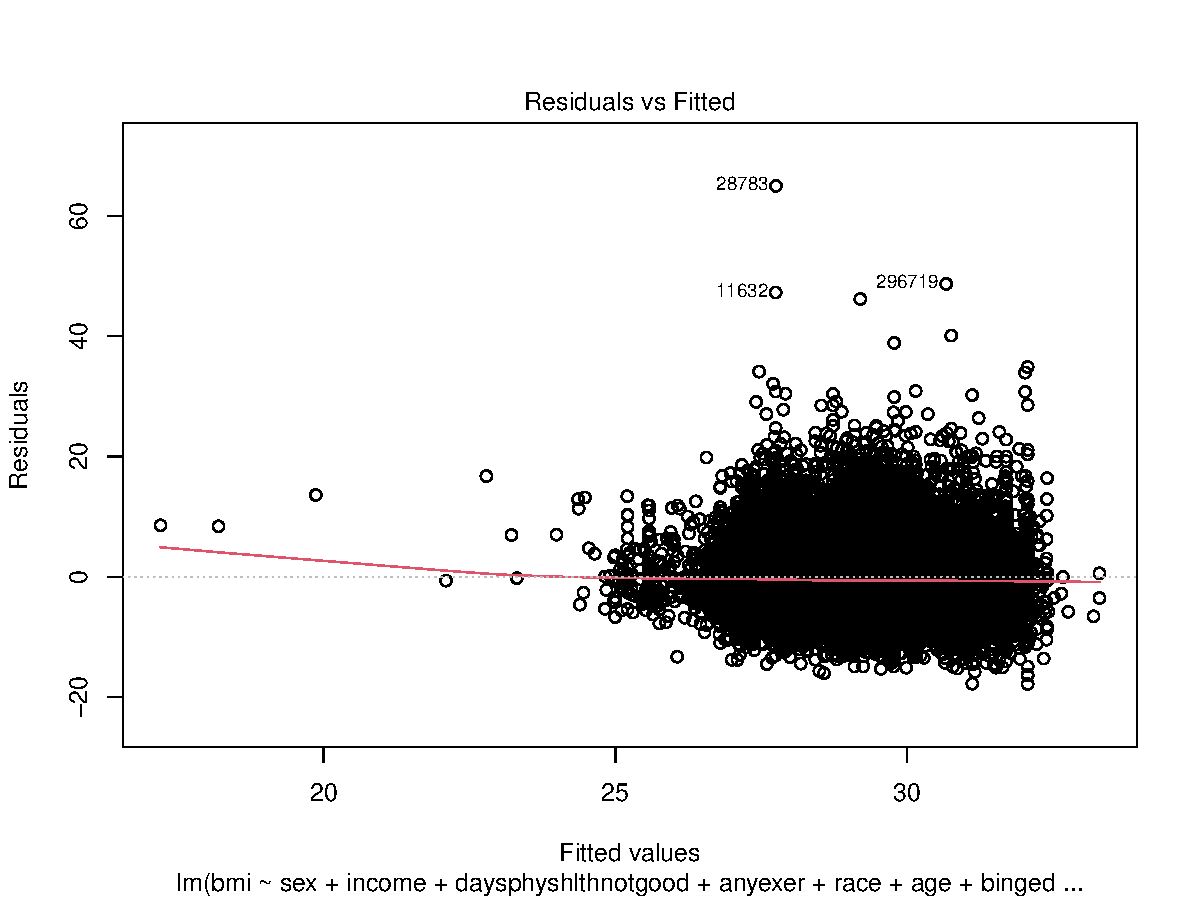
\includegraphics[width=0.6\linewidth,height=\textheight,keepaspectratio]{final-project_files/figure-pdf/unnamed-chunk-21-1.pdf}
\end{center}

\begin{center}
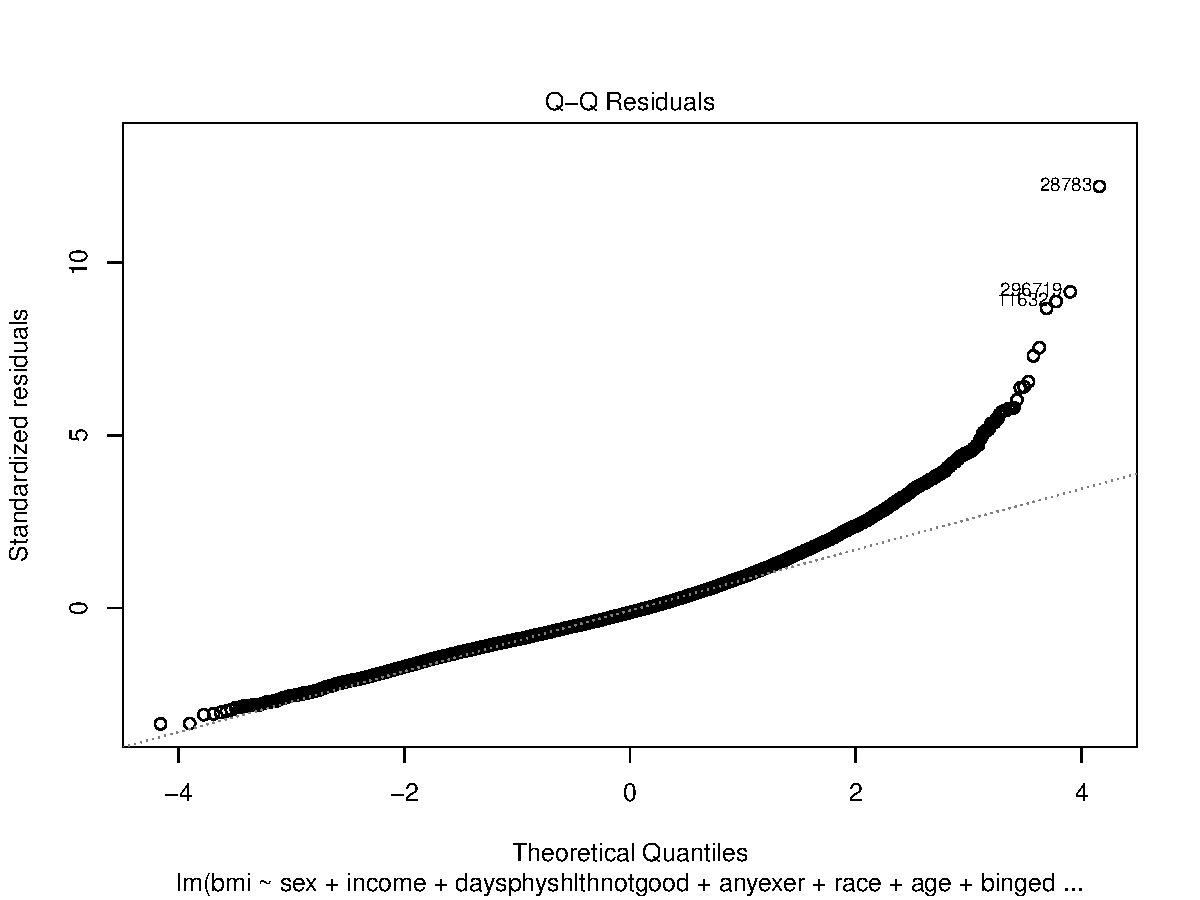
\includegraphics[width=0.6\linewidth,height=\textheight,keepaspectratio]{final-project_files/figure-pdf/unnamed-chunk-21-2.pdf}
\end{center}




\end{document}
